\section{Fundamento teórico}

Para comenzar se deben establecer unos parámetros para con la pala, ya que lo más básico de este trabajo empieza por determinar los efectos que produce la torsión en nuestra obtención de energía.

Es por ello que se determina que la pala de la turbina eólica es un \textbf{trapecio} cuya representación simplificada la vemos en la Figura \ref{fig:pala_simp}


\begin{figure}[H]
    \centering
    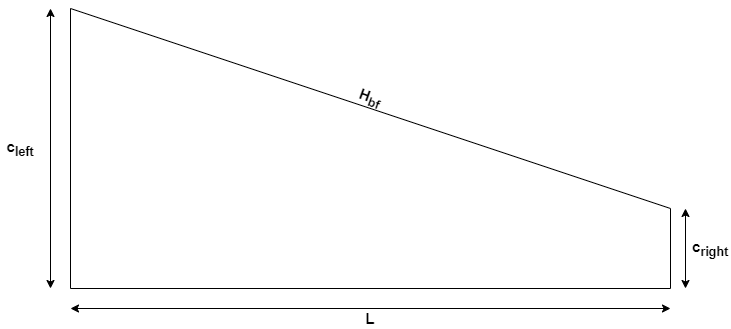
\includegraphics[width=0.7\textwidth]{images/pala simple.png}
    \caption{Representación de una pala de turbina eólica}
    \textit{Fuente: Elaboración propia}
    \label{fig:pala_simp}
\end{figure}



Lo siguiente que se debe tener presente es que se necesita también una representación de la pala de la figura \ref{fig:pala_simp} dividida en segmentos de igual largo para poder comprender el desarrollo que se realizará simulando una torsión, en la cual se girarán los segmentos un cierto ángulo los unos de los otros.

    \textbf{}
    \begin{figure}[H]
    \centering
    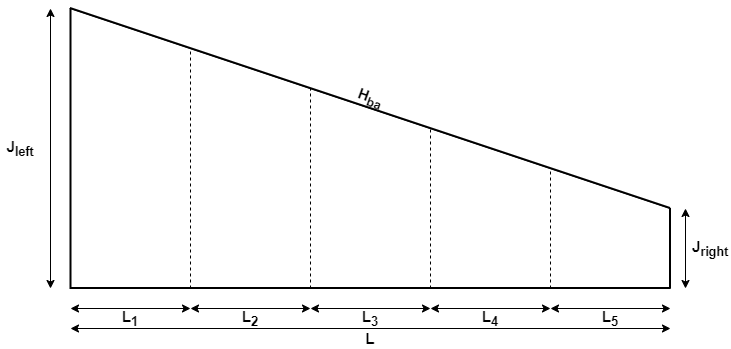
\includegraphics[width=0.7\textwidth]{images/pala simple segmentada.png}
    \caption{Representación de una pala de turbina eólica dividida en segmentos}
    \textit{Fuente: Elaboración propia}
    \label{fig:pala_dividida}
\end{figure}

Por simplicidad, la pala se dividirá únicamente en $N$ segmentos, en este caso 5. Aunque se mantenga este valor durante el trabajo y es probable que no cambie, se asociará a una variable en caso de que se quieran hacer pruebas mediante simulación en MATLAB más adelante. \\\\
    

La $L$ o \textit{longitud de pala}, vista en la Figura \ref{fig:pala_simp} es con la que se va a trabajar, por ello cada uno de los segmentos de la Figura \ref{fig:pala_dividida} tendrá el siguiente largo $\dfrac{L}{N} = \dfrac{L}{5}$ ya que se dividió $N$ número de veces. \\

Como se puede observar en la Figura \ref{fig:pala_dividida} cada segmento tiene una altura variable, esto se debe a la forma real de las palas, cuanto más cerca del buje de la turbina, mayor es el área del segmento. La altura en el centro de estos segmentos, conocida como $chord \text{ } line$ o $línea \text{ } de \text{ } cuerda$ se determinará mediante el preestablecimiento de una serie de datos y su desarrollo matemático relacionados con la pala completa.\\

Para el cálculo de la $línea \text{ } de \text{ } cuerda$ se requiere la realización de un desarrollo trigonométrico. 

\begin{figure}[H]
    \centering
    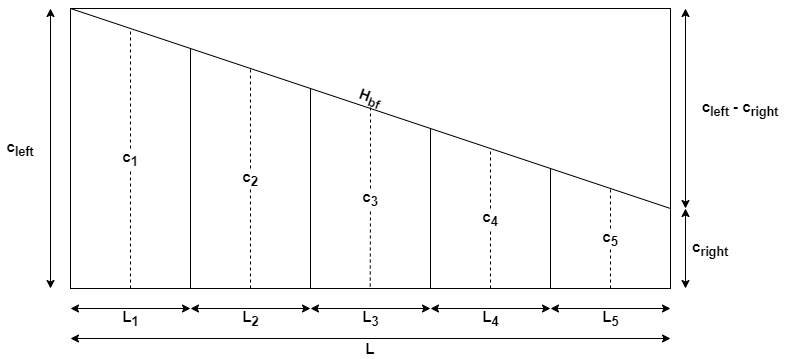
\includegraphics[width=0.9\textwidth]{images/planteo chord line.png}
    \caption{Representación parametrizada de la pala de una turbina eólica marina}
    \textit{Fuente: Elaboración propia}
    \label{fig:pala_desarrollo_chord}
\end{figure}



\begin{definicion}
En base a esta representación esquemática se puede deducir que:
$$ c_{left} = J$$
$$ c_{right} = J/D$$
$$ L_i = L/N$$
Donde,
\centering
J y D $\in \mathbb{Q+}$, \hspace{2pt} $J > D$, \hspace{2pt} $L_i$ := longitud del segmento,  $c_{left}$ := longitud simplificada del buje o hub de la pala y $c_{right}$ := longitud simplificada de la punta o tip de la pala, $i \in segmento$ y $segmento = \{1, ..., N\}$ 
\label{def_laterales_pala}
\end{definicion}


Ahora, una vez se tienen las variables básicas para conocer el resto de parámetros, se comienza con los cálculos.

\begin{definicion}
Con las variables formalizadas en la anterior definición, se define el valor $H_{bf}$ mediante el teorema de Pitágoras ya que el triángulo es rectángulo.

$$ H_{bf} = \sqrt{(c_{left} - c_{right})^{2} + L^{2}}$$
Donde,
\centering
$L$ := longitud de la pala, $H_{bf}$ := borde de fuga de la pala, $c_{left}$ := longitud simplificada del buje o hub de la pala y $c_{right}$ := longitud simplificada de la punta o tip de la pala.
\label{def_hipotenusa_pala}
\end{definicion}


A continuación, lo próximo que se debe obtener es el ángulo $\Phi$ o \textit{Ángulo de la línea del borde de arrastre de la pala de la turbina eólica}, para así conocer como decrece la $H_{bf}$ y mediante una relación trigonométrica extraída del artículo \cite{armenta2021predictive} poder obtener los valores de la \textit{Líneas de cuerda}.

\begin{figure}[H]
    \centering
    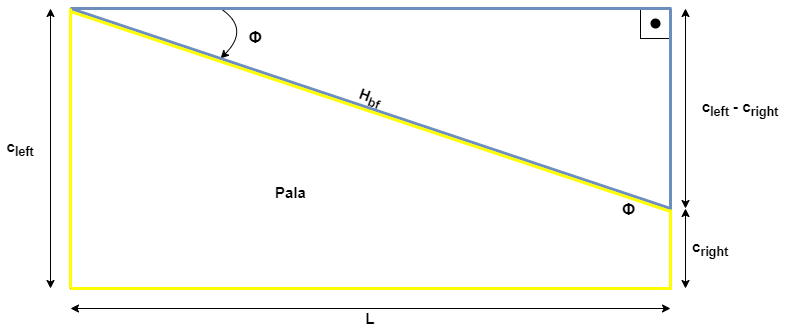
\includegraphics[width=0.9\textwidth]{images/triangulo sacar phi.drawio.png}
    \caption{Pala de la turbina en amarillo y triángulo usado para el cálculo de $\Phi$ en azul}
    \textit{Fuente: Elaboración propia}
    \label{fig:pala_calculo_phi}
\end{figure}

\begin{definicion}
En base a la figura \ref{fig:pala_calculo_phi} se puede deducir de tres formas por trigonometría el ángulo $\Phi$:
$$ \Phi = \arcsin{(\dfrac{c_{left} - c_{right}}{H_{bf}})} $$
$$ \Phi = \arccos{(\dfrac{L}{H_{bf}})} $$
$$ \Phi = \arctan{( \dfrac{\sin{(\dfrac{c_{left} - c_{right}}{H_{bf}})}}{\cos{(\dfrac{L}{H_{bf}})}} ) } $$
Donde,
\centering
$L$ := longitud de la pala, $H_{bf}$ := borde de fuga de la pala, $c_{left}$ := longitud simplificada del buje o hub de la pala y $c_{right}$ := longitud simplificada de la punta o tip de la pala.
\label{def_angulo_phi}
\end{definicion}


El siguiente paso para calcular las $líneas \text{ } de \text{ } cuerda$ se basa en aislar trapecios mas pequeños de los que se han obtenido todos los datos menos el valor de su base menor que se tendrá que calcular, siendo este equivalente a $c$.\\

\begin{definicion}
Variables necesarias para el cálculo de las líneas de cuerda.

$$ altura_i = \dfrac{(2i - 1) \cdot L}{2N}$$
$$ diagonal_i = \dfrac{(2i - 1) \cdot H_{bf}}{2N}$$

Donde,
\centering
$L$ := longitud de la pala, $H_{bf}$ := borde de fuga de la pala, $altura_i$ := Longitud de la pala fragmentada para el cálculo de la línea de cuerda, $H_{bf}$ := Hipotenusa del borde de fuga fragmentada para el cálculo de la línea de cuerda, $i \in segmento$ y $segmento = \{1, ..., N\}$
\label{def_variables_fragmentadas}
\end{definicion}

Por último y una vez definido todo lo necesario, se pasa al cálculo mediante el cual se obtiene el valor de todas y cada una de las $líneas \text{ } de \text{ } cuerda$ de la pala con la que se está trabajando.

\begin{definicion}
Primero se obtiene la diferencia mediante Pitágoras entre la base mayor y la menor, definida como $x_i$, después la resta de la base mayor y esta diferencia.

$$ x_i = \sqrt{diagonal_i^{2} - altura_i^{2}}$$

$$ c_i = c_{left_i} - x_i $$

Donde,
\centering
$L$ := longitud de la pala, $H_{bf}$ := borde de fuga de la pala, $altura_i$ := Longitud de la pala fragmentada para el cálculo de la línea de cuerda, $H_{bf}$ := Hipotenusa del borde de fuga fragmentada para el cálculo de la línea de cuerda, $i \in segmento$ y $segmento = \{1, ..., N\}$
\label{def_chord_line}
\end{definicion}

La siguiente figura, ilustra el ejemplo en el que para las definiciones \ref{def_variables_fragmentadas} y \ref{def_chord_line} el valor de $i$ es igual a 3. Obteniendo así $c_3$. En verde el trapecio y en magenta el triángulo del que restamos el cateto a la base mayor del trapecio.

\begin{figure}[H]
    \centering
    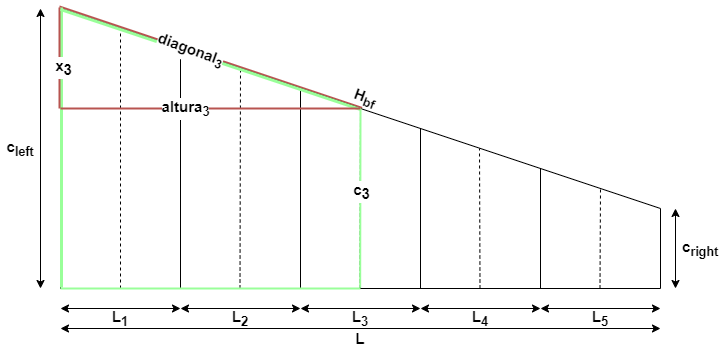
\includegraphics[width=0.9\textwidth]{images/Trapecio calculo x.png}
    \caption{Pala de la turbina en amarillo y triángulo usado para el cálculo de $\Phi$ en azul}
    \textit{Fuente: Elaboración propia}
    \label{fig:pala_calculo_phi}
\end{figure}


Una vez se ha obtenido el valor buscado $c_i$, se deberá definir todos los laterales de los segmentos de la pala, para así poder operar con ellos en pos de conseguir el área de cada uno de ellos. Esto ya fue desarrollado en el artículo \cite{armenta2021predictive}, pero en aquel caso fue usado para comprobar el error que suponía usar un rectángulo en vez de una pala simplificada. En este caso se parte directamente de la pala simplificada para evitar correcciones de errores mas adelante y porque el cálculo que se debe realizar con respecto a la obtención de energía no es tan profundo y complicado como en el artículo \cite{armenta2021predictive}. Además remarcar que para las deducciones y cálculos anteriores se bebió de este desarrollo.


\begin{definicion}
En base a esta representación esquemática y mediante relaciones trigonométricas obtuvieron:
$$ c_{left_i} = c_i + (\dfrac{L_i}{2}) \tan \varPhi$$
$$ c_{right_i} = c_i - (\dfrac{L_i}{2}) \tan \varPhi$$
Donde,
\centering
$i \in segmento$ y $segmento = \{1, ..., N\}$
\label{def:laterales_segmento}
\end{definicion}

Al igual que se deduce en el artículo \cite{armenta2021predictive}, con los datos obtenidos de los laterales de cada segmento, se puede trabajar con una forma de trapecio y encontrar el área de los segmentos que se definieron en la Figura \ref{fig:pala_dividida}.\\

Aparte, con esta definición se ve que en la Figura \ref{fig:pala_desarrollo_chord} los valores de $c_{leftt_i}$ y de $c_{right_i}$ que se observan, realmente serían equivalentes a $c_{left_1}$ y a $c_{right_5}$, respectivamente. Estos son definidos a priori debido a su importancia para caracterizar la pala de manera correcta y con las dimensiones que el usuario desee.

\begin{definicion}
Se determina el área de los segmentos:
$$ S_{i} = \dfrac{(c_{left_i} + c_{right_i})}{2N} \cdot L_i $$
Donde,
\centering $i \in segmento$, $segmento = \{1, ..., N\}$ y $S_i$ := Área del segmento.
\label{def:area_segmentos}
\end{definicion}







%Sujeto a cambios todo lo que va a continuación
A continuación, se supone que los segmentos están ensartados por una línea imaginaria que ayudará al estudio de la torsión mediante giros de los segmentos alrededor suya.


\subsection{Estudio del torque con giro inicial}
\label{section:torque_giro_inicial}

Se han presentado algunos de los conceptos básicos, ahora se introduce el ángulo $ \theta_1 $, que es la constante definida como el \textit{giro inicial} que sufrirán todos y cada uno de los segmentos que son paralelos al plano horizontal, desde el cual se presenta el viento que incidirá en nuestra pala.\\

En esta primera sección se estudiará qué ocurre en término de fuerzas, torque y momento cuando se gira toda nuestra pala únicamente el ángulo de giro inicial $ \theta_1 $, sin necesidad de segmentarla, tal y como se aprecia en la figura \ref{fig:pala_simp}. \\


Es cierto que se podría no girar la pala este giro inicial $ \theta_1 $, pero por comodidad de cálculo y para establecer un ángulo de ataque del viento paralelo a la horizontal se realizará de esta manera.\\


Al haber inclinado todos los segmentos un ángulo $ \theta_1 $ se genera la situación en la que el viento incide en el centro del segmento con el mismo ángulo con el que se inclina la pala. \\

    \textbf{}
    \begin{figure}[H]
    \centering
    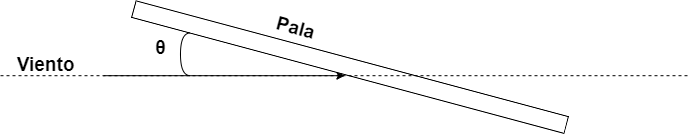
\includegraphics[width=0.8\textwidth]{images/dibujo angulo ataque.drawio.png}
    \caption{Ángulo de ataque del viento con respecto a la pala}
    \textit{Fuente: Elaboración propia}
    \label{fig:dibujo_angulo_ataque}
\end{figure}

La fuerza del viento que incide en la pala se puede descomponer en 2, la tangencial y la normal. \\

    \textbf{}
    \begin{figure}[H]
    \centering
    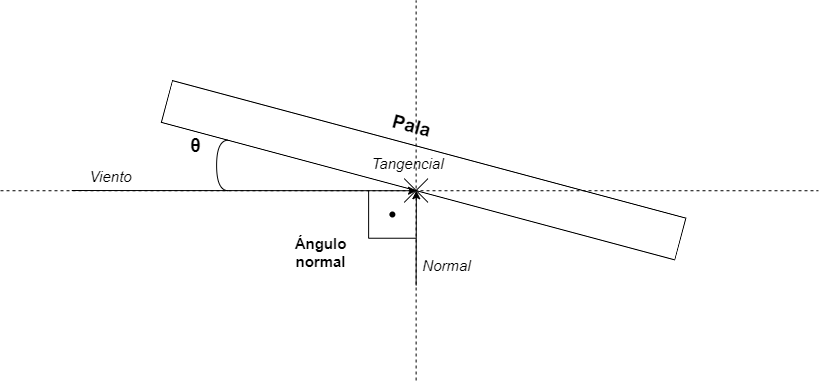
\includegraphics[width=1\textwidth]{images/dibujo fuerzas.drawio.png}
    \caption{Descomposición de vectores de fuerzas}
    \textit{Fuente: Elaboración propia}
    \label{fig:dibujo_fuerzas}
\end{figure}


Como se puede ver en la figura \ref{fig:dibujo_fuerzas} el vector fuerza normal es perpendicular al ángulo de ataque del viento, mientras que el vector fuerza tangencial recorre de manera paralela la línea central de la pala.

